% -------------------------------------------------------------------------------------------------------
%-----------------------------CONSULTA DE PLANES DE ESTUDIO---------------------------------
% -------------------------------------------------------------------------------------------------------

\chapter{Gestión de Plan de Estudios}
\section{Consulta de Planes de Estudios}
Cuando el Jefe de Innovación Educativa da clic en la sección de \textbf{Gestionar Planes de Estudio} aparecerá la siguiente pantalla:

% Imagen menu

\begin{figure}[!hbtp]
	\centering
	\hypertarget{consultarPE}{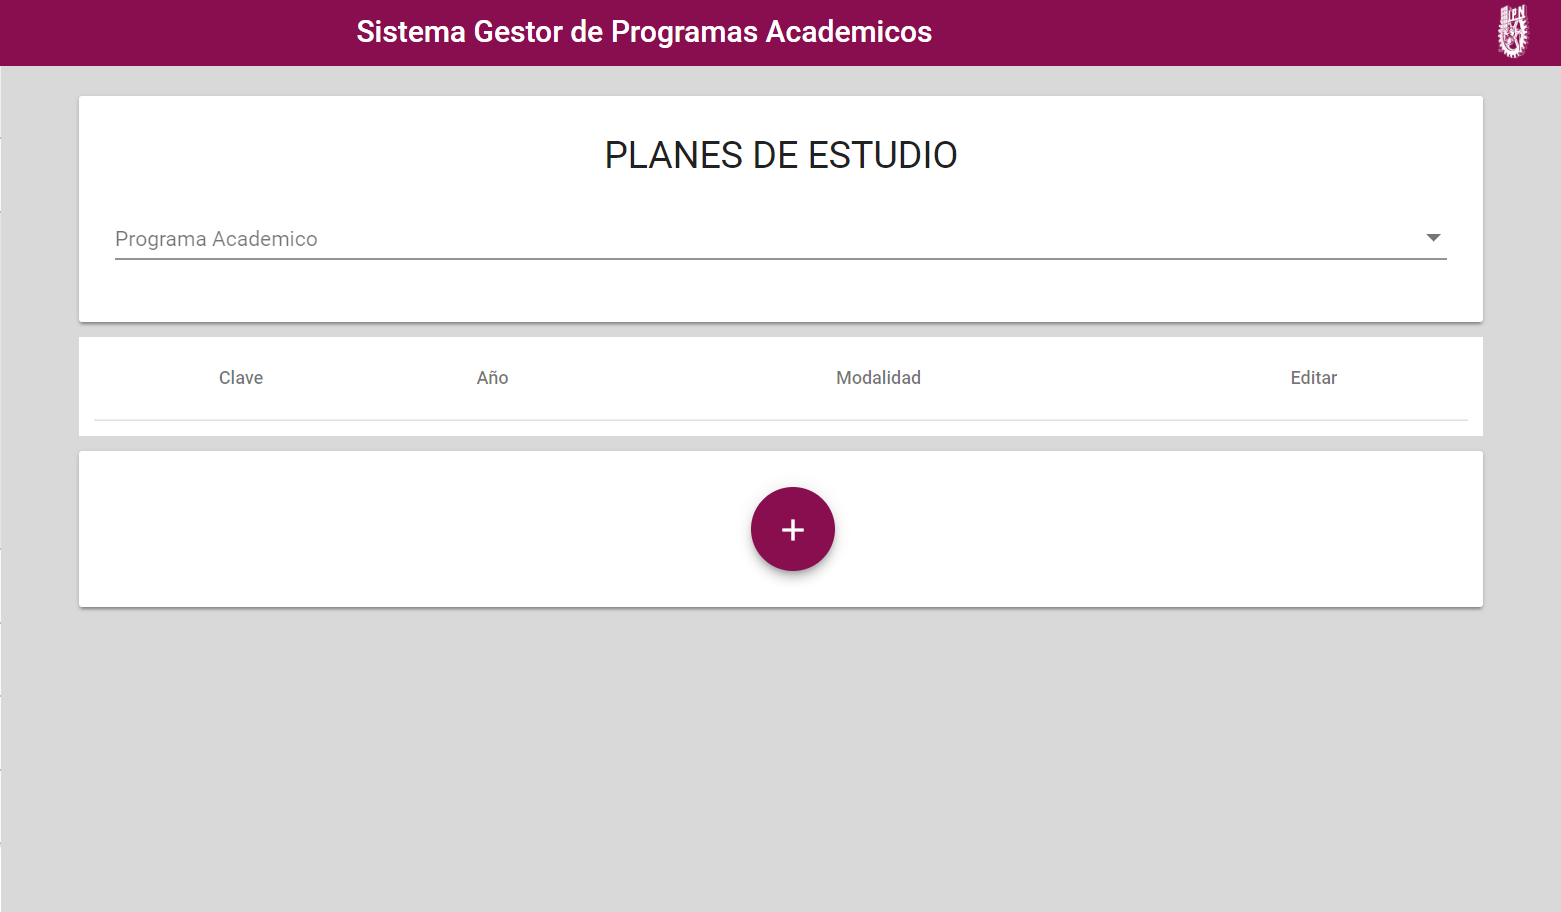
\includegraphics[width=0.7\linewidth]{images/SP4-GPE/consultar}}
	\caption{Pantalla para Planes de Estudio}
	\label{consultarPE}
\end{figure}

En donde aparecerá, de forma predeterminada, todos los Planes de Estudios a su cargo registrados en el sistema al momento. Tendrá a su disposición dos funciones:

\subsection{Buscar Planes de Estudio según su cargo}

Para ello, el Jefe de Innovación Educativa tendrá que seleccionar el Programa Académico que desea consultar en el siguiente componente:

\begin{figure}[!hbtp]
	\centering
	\hypertarget{academico}{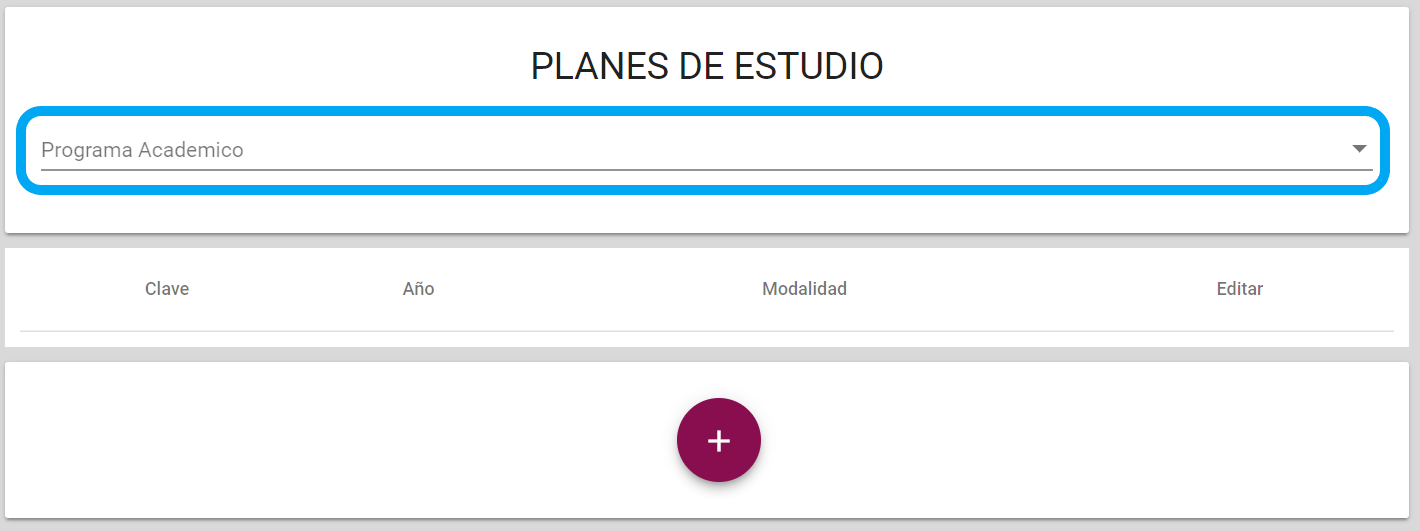
\includegraphics[width=0.7\linewidth]{images/SP4-GPE/programa}}
	\caption{Selección de Programa Académico}
	\label{academico}
\end{figure}

\begin{figure}[!hbtp]
	\centering
	\hypertarget{academico2}{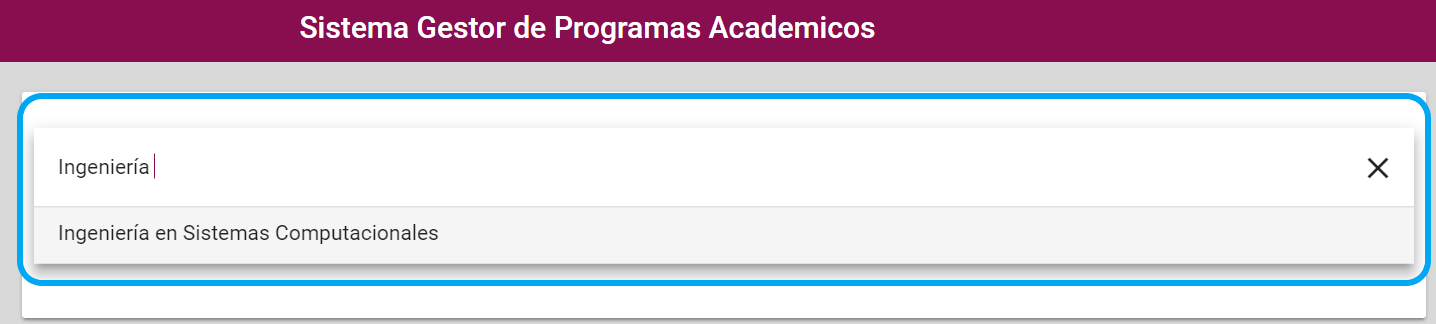
\includegraphics[width=0.7\linewidth]{images/SP4-GPE/programaD}}
	\caption{Despliegue de Programas Académicos}
	\label{academico2}
\end{figure}

A continuación el sistema mostrará todos los Planes de Estudios que tengan el Programa Acádemico seleccionado.
\begin{figure}[!hbtp]
	\centering
	\hypertarget{planes}{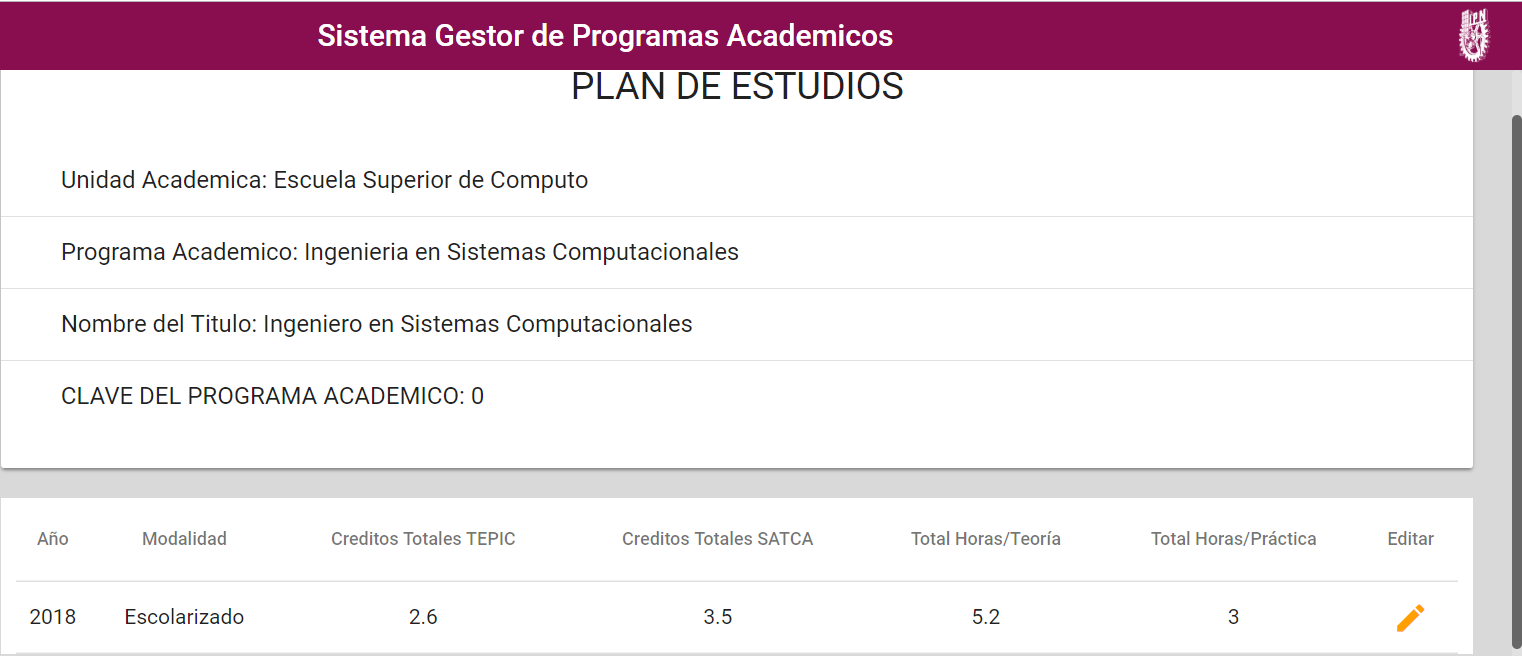
\includegraphics[width=0.7\linewidth]{images/SP4-GPE/planes}}
	\caption{Planes de Estudios Encontrados}
	\label{planes}
\end{figure}
\newpage
\section{Editar Planes de Estudios}

Para ello, el Jefe de Innovación Educativa tendrá que dar clic en el boton \IUbutton{icono de lapiz amarillo} que esta al lado del Plan de Estudio que desea modificar. Al hacer esto, el sistema redireccionará al usuario a la pantalla de \hyperlink{editarPE}{\textit{Editar Plan de Estudio}}.

\begin{figure}[!hbtp]
	\centering
	\hypertarget{editar}{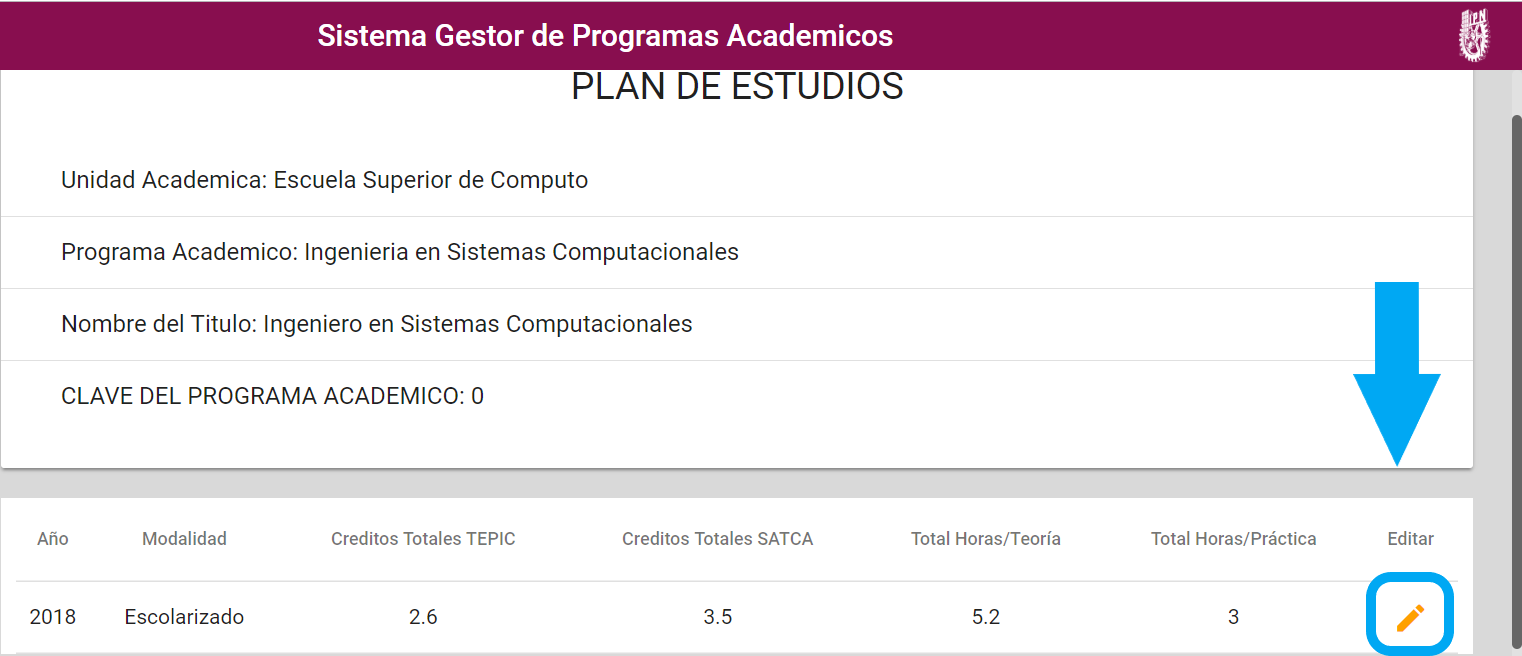
\includegraphics[width=0.7\linewidth]{images/SP4-GPE/editarC}}
	\caption{Botón Editar Plan de Estudio}
	\label{editar}
\end{figure}
\newpage
\begin{figure}[!hbtp]
	\centering
	\hypertarget{editarPE}{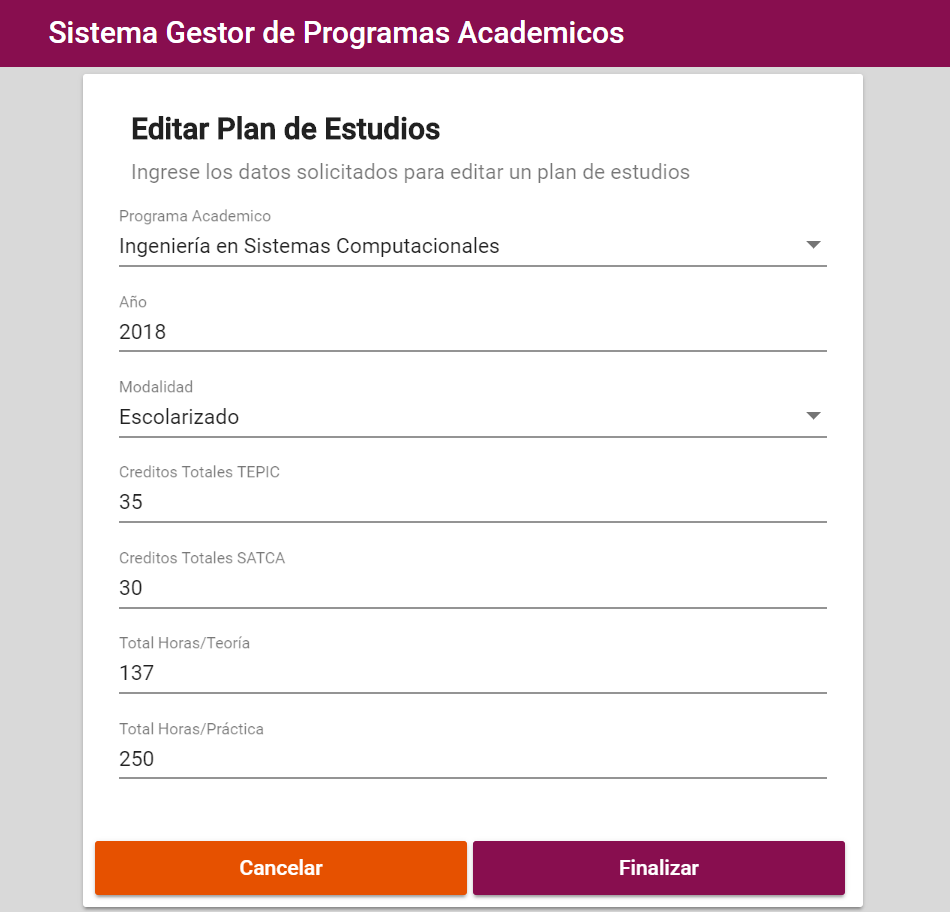
\includegraphics[width=0.7\linewidth]{images/SP4-GPE/editarPE}}
	\caption{Pantalla para la edición de Planes de Estudios}
	\label{editarPE}
\end{figure}

En donde se cargarán los datos del Plan de Estudio seleccionado en la pantalla de \hyperlink{consultarPE}{\textit{Consultar Planes de Estudios}} y llenará el formulario.
\newpage
A continuación, el usuario puede modificar todos los campos del Plan de Estudio.
\begin{figure}[!hbtp]
	\centering
	\hypertarget{modif}{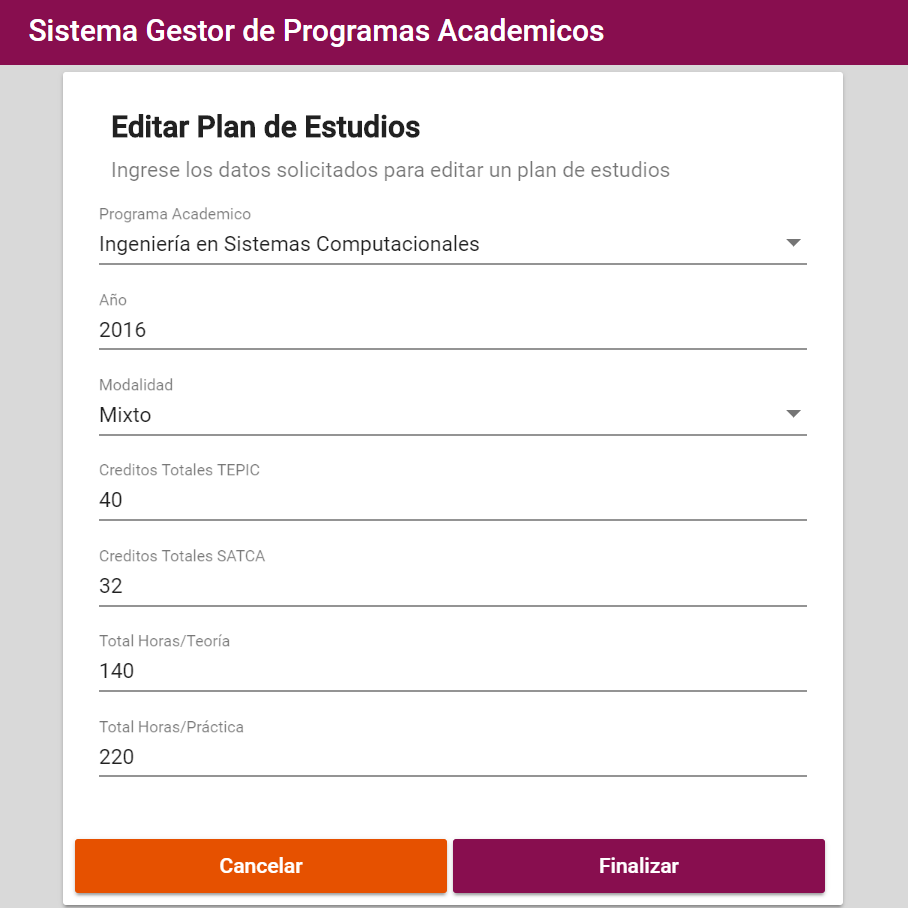
\includegraphics[width=0.7\linewidth]{images/SP4-GPE/editarPE1}}
	\caption{Datos del Plan de Estudio modificados}
	\label{modif}
\end{figure}

 Si el Jefe de Innovación Educativa da clic en el botón \IUbutton{Cancelar} sin haber concluido la edición del Plan de Estudio:

\begin{figure}[!hbtp]
	\centering
	\hypertarget{cancel2}{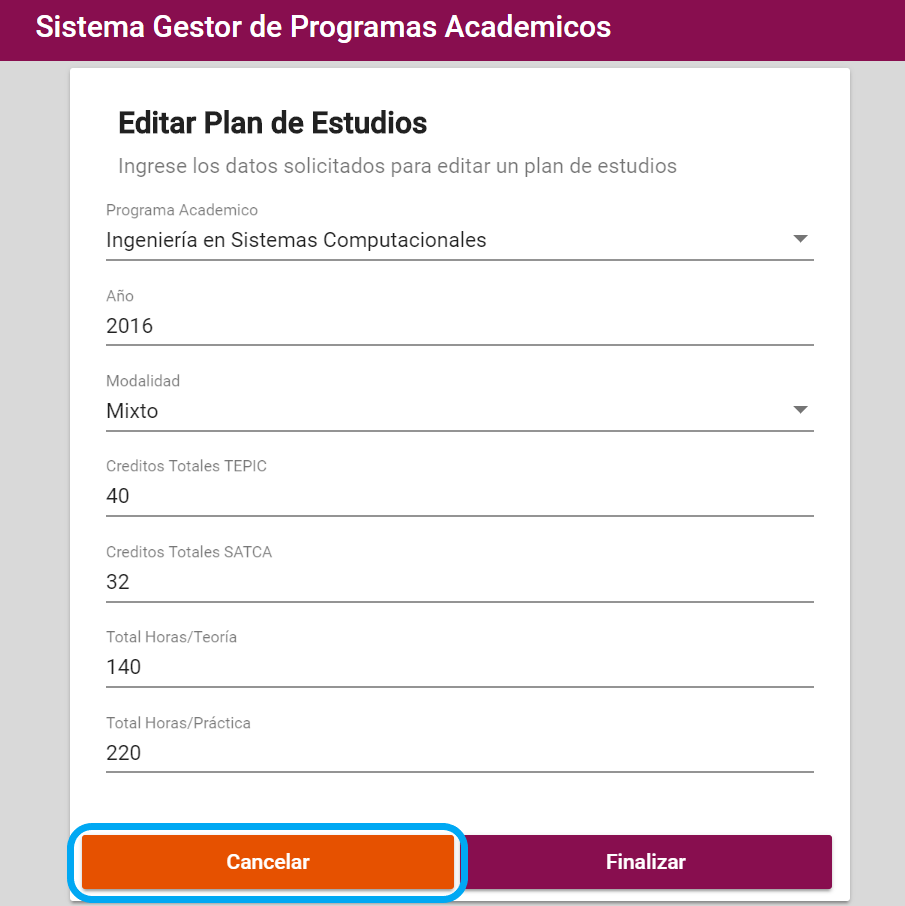
\includegraphics[width=0.7\linewidth]{images/SP4-GPE/cancelarPE}}
	\caption{Botón ''Cancelar''}
	\label{cancel2}
\end{figure}

El sistema mostrará el siguiente mensaje:
%Imagen MSG30

Para confirmar, el usuario debe dar clic en el botón  \IUbutton{Si}, y el Plan de Estudio no será modificado.\\

Para cancelar, el usuario debe dar clic en botón  \IUbutton{No}, el mensaje se cerrará y continuaremos en el formulario. Aqui el Jefe de Innovación Educativa puede terminar la edición del Plan de Estudio.\\
\newpage
Una vez modificados los datos, deberá de dar clic en el botón  \IUbutton{Registrar}.
\begin{figure}[!hbtp]
	\centering
	\hypertarget{btnfin}{
\includegraphics[width=0.7\linewidth]{images/SP4-GPE/editarPER}}
	\caption{Botón ''Registrar''}
	\label{btnfin}
\end{figure}

Si no hubieron errores, el sistema muestra el siguiente mensaje:
%Imagen MSG27

Al dar clic en en botón  \IUbutton{Aceptar}, el sistema redireccionará al usuario a la pantalla de \hyperlink{consultarPE}{\textit{Consultar Planes de Estudis}}, en donde podrá ver las modificaciones del Plan de Estudios.\\
\newpage
\subsection{Posibles errores}

\begin{itemize}
	\item Problemas con la conexión o el sistema

	Si al momento de acceder a la pantalla de \hyperlink{editarPE}{\textit{Editar Plan de Estudio}} o al intentar modificar un Plan de Estudio, aparece alguno de los siguientes mensajes:

	% Imagen MSG7 Y MSG25

	Significa que existió un error de conexión o del sistema. Al dar clic en en botón  \IUbutton{Aeptar}, el sistema redireccionará al usuario a la pantalla de \hyperlink{consultarPE}{\textit{Consultar Planes de Estudios}}. Debe esperar a que la página este disponible o intentar acceder nuevamente.

	\item Campos vacíos al momento de modificar el Plan de Estudio

	Si el Jefe de Innovación Educativa dejo en blanco algún campo del formulario, y posteriormente dio clic en el botón  \IUbutton{Registrar}, el sistema mostrará el siguiente mensaje:

	% Imagen MSG32

	Al dar clic en botón  \IUbutton{Aceptar}, el mensaje se cerrará y regresaremos al formulario, en donde el usuario deberá llenar el o los campos que dejo vacío. Si se continúan dejando campos en blanco y dando clic en el botón  \IUbutton{Registrar}, aparecerá nuevamente el mensaje, hasta que todos los campos sean llenados.

	\item Los campos ingresados no son válidos

	Si al momento de dar clic en el \IUbutton{Registrar} aparece el siguiente mensaje:
	% Imagen MSG20

	Significa que la composición de los datos ingresados en el formulario no es la correcta, verifíquelos e intente de nuevo.

\end{itemize}
